% Use either your LaTeX editor or latexmk to compile.

\documentclass[a4paper, 12pt]{article}

% Document quality things
\usepackage[utf8]{inputenc}
\usepackage{microtype, xcolor}
\usepackage{url, hyperref}
\hypersetup{colorlinks=true, linkcolor=blue, citecolor=black, urlcolor=blue}

% Image-related packages
\usepackage{graphicx}
\usepackage{float}
\graphicspath{ {./ui-design-mockups/} }
\usepackage[font=small,skip=5pt]{caption}

% Setting margins
\usepackage[a4paper, left=2cm, right=2cm, top=1.75cm, bottom=1.75cm, includefoot]{geometry}

% Table helper packages
\usepackage{multirow, multicol}
\usepackage{makecell}
\usepackage{array}
%\usepackage{tabularx} % Not needed currently, but has a few nice options
\usepackage{wrapfig} % Floating figures/tables

% Prevents spamming tedious newlines everywhere, also disables auto indentation, etc.
\usepackage[skip=0.75\baselineskip plus 2pt]{parskip}

% Self-explanatory
\usepackage{titlesec}
\titleformat{\section}[block]{\normalfont\scshape\Large}{\thesection}{1em}{}
\titleformat{\subsection}{\normalfont\large}{\thesubsection}{1em}{}

% Referencing
\usepackage[backend=bibtex, style=numeric-comp, sorting=none]{biblatex}
\addbibresource{bibliography.bib}

\begin{document}
    
    % Header Table
    \begin{table}[h!]
        \renewcommand{\arraystretch}{3}
        \centering
        \begin{tabular}{ | >{\raggedleft\arraybackslash}m{3cm} l >{\raggedleft\arraybackslash}m{3cm} m{3cm} | }
            \hline
            \Huge CS 102 & \textit{Spring 2020/21} & \multirow{2}{*}{\makecell{Project\\Group}} & \multirow{2}{*}{\textbf{\Huge G2C}} \\
            \makecell[r]{Instructor:\\Assistant:} & \makecell[l]{\textbf{Aynur Dayanık}\\\textbf{Haya Shamim Khan Khattak}} & & \\
            \hline
        \end{tabular}
    \end{table}
    
    % Grading Table
    \begin{table}[h!]
            \renewcommand{\arraystretch}{1.4}
            \centering
            \footnotesize
            \begin{tabular}{ l p{1.5cm} | p{1.5cm} | }
                \hline
                \multicolumn{1}{|c|}{\textbf{Criteria}} & \multicolumn{1}{c|}{\textbf{TA/Grader}} & \multicolumn{1}{c|}{\textbf{Instructor}} \\ \hline
                \multicolumn{1}{|p{10.5cm}|}{Presentation} &  &  \\[10ex] \hline
                \multicolumn{1}{r|}{\textbf{Overall}} &  &  \\
                \cline{2-3}
            \end{tabular}
    \end{table}
    
    % Project Information Header
    {\centering\Huge \bfseries \raisebox{0.5ex}{\texttildelow} LabConnect \raisebox{0.5ex}{\texttildelow} \par}
    
    \begin{table}[h!]
        \renewcommand{\arraystretch}{1.4}
        \centering
        \small
        \begin{tabular}{ r l }
            \textbf{Borga Haktan Bilen} & 22002733 \\
            \textbf{Vedat Eren Arıcan} & 22002643 \\
            \textbf{Berkan Şahin} & 22003211 \\
            \textbf{Berk Çakar} & 22003021 \\
            \textbf{Alp Ertan} & 22003912 \\
        \end{tabular}
    \end{table}
    
    % Document Type Header Table
    \begin{table}[h!]
        \renewcommand{\arraystretch}{1.5}
        \centering
        \begin{tabular}{ |>{\centering\arraybackslash}m{15.15cm}| }
            \hline
            \Large \textbf{UI Design Report} \\
            \small (version 1.0) \\
            \small \textbf{\today} \\
            \hline
        \end{tabular}
    \end{table}
    
    % Document begins here...
    
    \section{Introduction to LabConnect}
    
    LabConnect is a developing project that aims to make education more productive for students,
    and more efficient for teaching staff, among other benefits. The feature list compiled for the
    sake of this goal includes items such as:
    \begin{itemize}
        \item Queueing system for live sessions to optimize wait times and student-TA communication
        \item Dashboard designed with a pragmatist mindset, to lessen confusion as much as viable
        \item Instructor panel where new assignments can be added with great flexibility
        \item Analysis view for students and teaching staff alike, to monitor course progress
        \item Announcements board where the teaching staff can reach out to students with ease
        \item Simple one-to-one messaging capability for the sake of light written communication
        \item Note-taking panel for students to take concise notes regarding individual assignments
        \item Detailed view of submission versions where students and the teaching staff can observe
            automated testing results
    \end{itemize}
    
    Though the above is not an exhaustive list of features, it does nonetheless capture the gist of the features
    this project proposes in order to undertake its goal of optimizing the assignment portion of
    a computer science course. For a more extensive summary of this project, refer to the requirements report published earlier.
    
    \section{Disclaimer Regarding the UI Design Report}
    
    The document herein contains details and illustrations from 13 application views in total, but certain disclaimers have to be made
    regarding the accuracy of these illustrations.
    LabConnect is planned to be a web application, built with established modern web design paradigms in mind. However, web pages,
    particularly those that strive to be designed responsively for the sake of usability on a distinct range of devices, are
    not easy to make \emph{static} prototype designs of. Along with this factor, another aspect affecting the UI design process is the fact
    that as LabConnect is an application with a large volume of interaction between people, which may take place at severely
    differing times, an unavoidable need to display certain elements only in very specific instances appears. In other words, the project
    at hand is of such nature that it cannot be \emph{accurately} put on display before an actual development of the interface, via
    the use of dynamic web technologies such as CSS and JavaScript, is in process. 

    As a side note, the development of the interface also depends directly on the implementation of the feature set,
    as the need for elements on the page will originate from the structures designed on the server application side of the project, which
    are highly liable to change as the back-end code undergoes development. An example of this phenomenon is the analysis view presented to the users,
    which is dependent highly on core features being implemented first, because only then can the data to be put on display be ascertained,
    and the interface thereof finalized.
    
    The UI design of LabConnect was completed with the above considerations in mind, which is to mean that the design was developed
    for the sake of having a guide to refer to when the necessity arises, rather than being developed for the impractical sake of being an accurate
    finalized version of the interface. We believe that this approach will prove to be more advantageous in the long term.
    
    \pagebreak
    
    \section{Map of the Application's Views}
    
    
    
    
    % TODO Add a "sitemap" of pages here, as seen on the document on a.dayanik's website.
    
    
    
    
    \pagebreak
    
    \section{User Interface Designs of Application Views}
    
    \subsection{User-agnostic Views}
    
    This subsection illustrates the pages of LabConnect that are intended to remain mostly unchanged regardless of the user's account level in the system
    (i.e., student, TA, instructor). Having certain user-agnostic views may help to make the interface easier to maintain, similar to how
    reusing existing code is often advised.
    
    \subsubsection{Login}
    
    \begin{figure}[H]
        \centering
        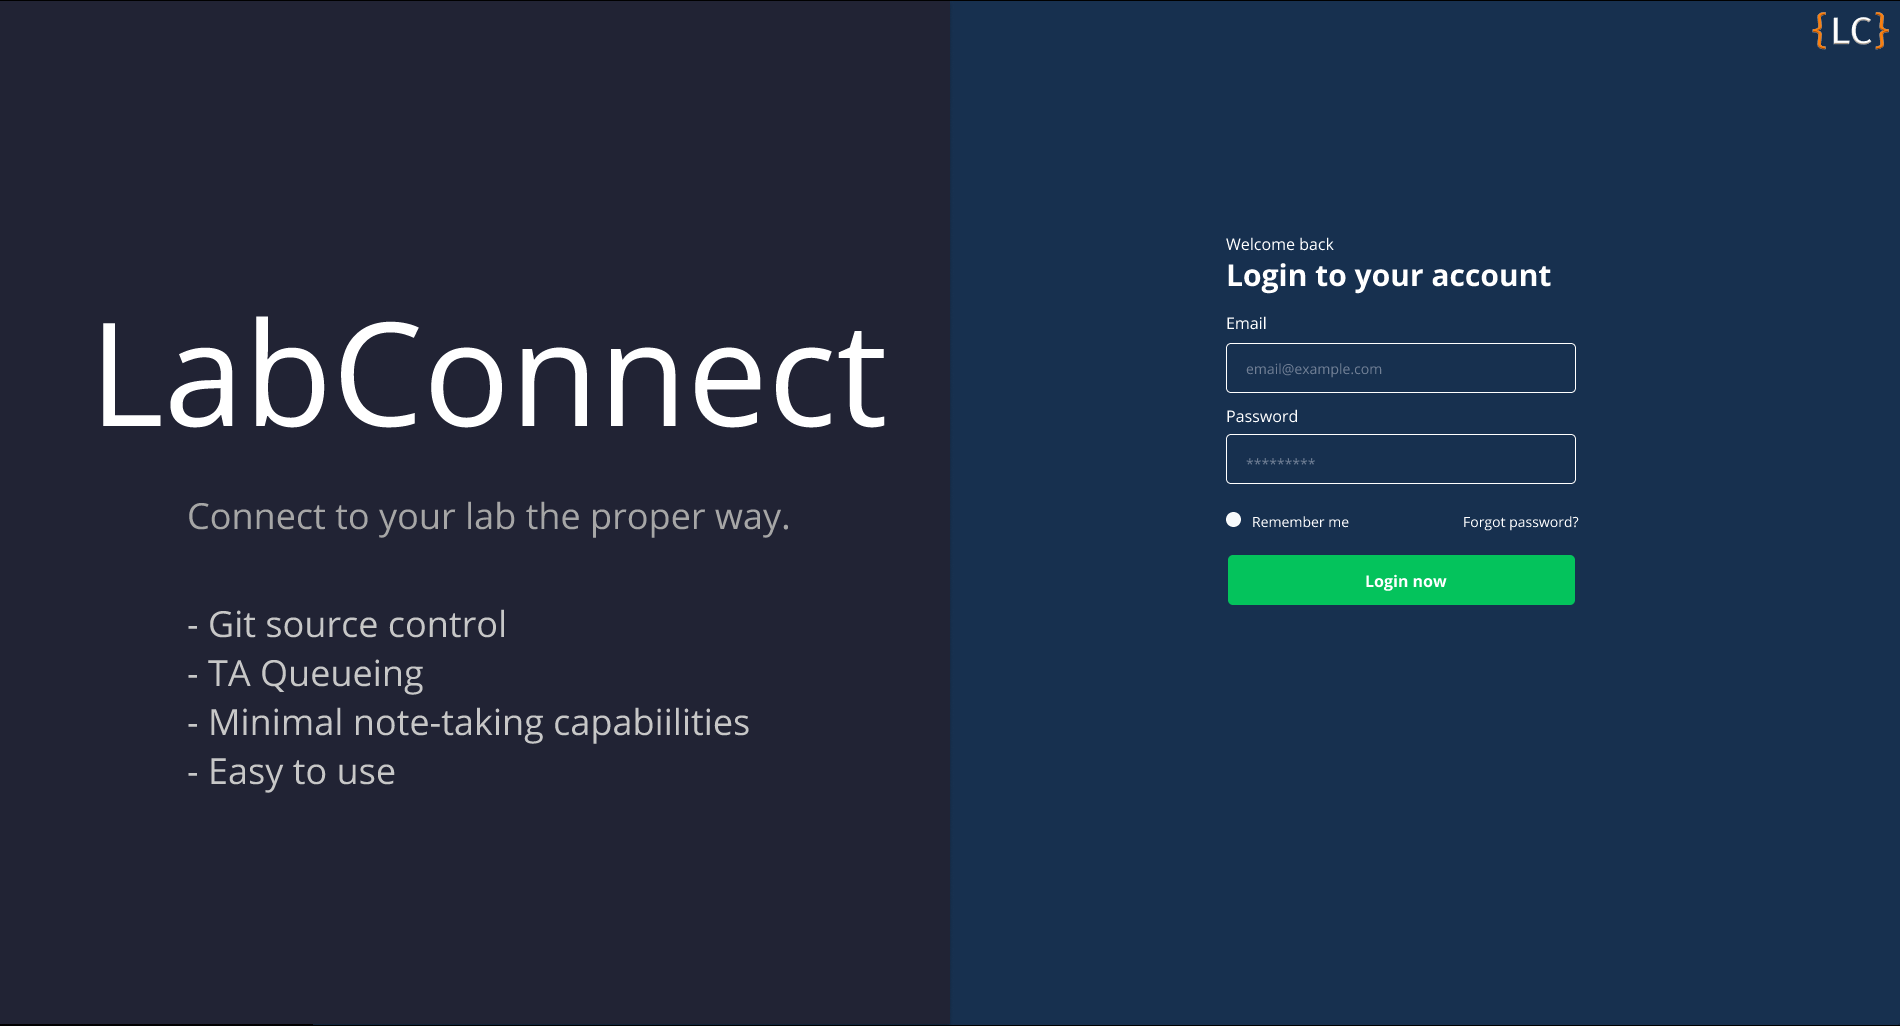
\includegraphics[width=\textwidth]{login}
        \caption{Complete view of the login UI}
        \label{fig:login_full}
    \end{figure}
    
    The view seen above in Figure \ref{fig:login_full} is the page every guest user will see upon visiting the website.
    On the left, a concise preview as to what the project is about, and is capable of, is provided.
    The features are also listed in order to give the user the ability to understand the inner workings of the
    system better, in case it may offer them a better experience utilizing the system later on.
    On the right, a similarly concise login panel is provided, with all of the common and basic features
    such as password recovery and a ``Remember me'' option.
    
    It is noteworthy that the guest user is not given a choice to register a new account.
    The reason is that, for the time being, the user database is planned to be modified by the administrators of the system directly.
    The users are intended to login once they have been shared the credentials created for them.
    
    \pagebreak
    
    \subsubsection{Dashboard}
    % Beware:
    % This "Dashboard" section is pretty troublesome with its layout.
    % It seems as if changing a word in here might have the potential of breaking things.
    % If you don't absolutely have to, refrain from modifying anything within
    % this section.
    
    \begin{figure}[H]
        \centering
        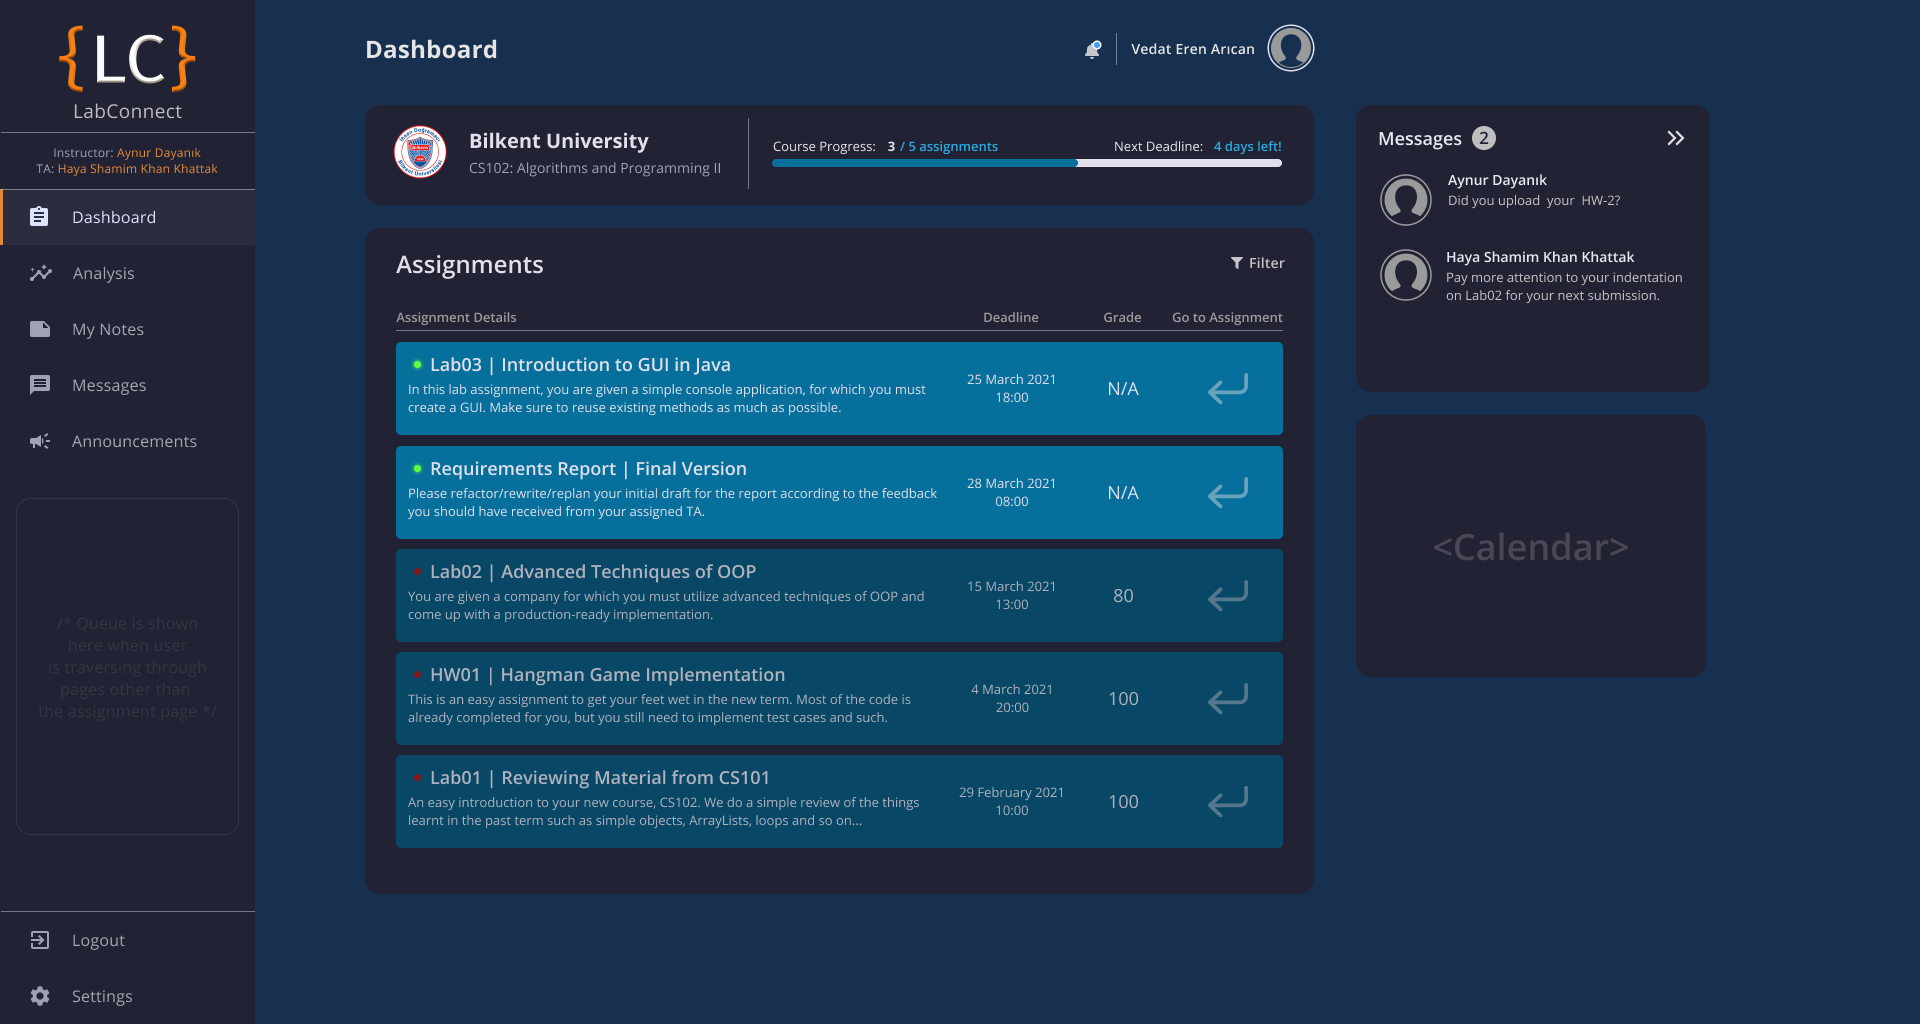
\includegraphics[width=\textwidth]{main_dashboard}
        \caption{Complete view of the dashboard UI}
        \label{fig:dashboard_full}
    \end{figure}
    
    The view above in Figure \ref{fig:dashboard_full} is the page every logged in user will see as their `homepage".
    The goal is to provide the user with a simple and tidy overview of things requiring their attention.
    The main two panels, unique to the page, are located in the center column: A list of all assignments and a small
    status panel at the top of the screen. The assignment list panel is the main navigation method into each individual
    assignment. Certain details of each assignment are provided on this page, however, the user needs to click on an
    assignment in order to visit a page with more details and features. To make it clear that the assignment items are
    to be clicked on, an entrance symbol is provided on the rightmost side of the item.
    The rest of the elements visible on this page are recurrent throughout most, if not all, of the other pages.
    As such, their significance and properties will be elaborated on in the following paragraph.
    
    \begin{wrapfigure}[15]{r}{0.34\textwidth}
        \centering
        \vspace{-15pt}
        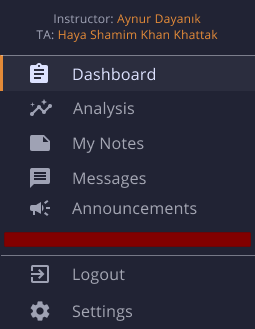
\includegraphics[width=0.34\textwidth]{navbar_short}
        \caption{Navigation bar, shortened for illustration purposes}
        \label{fig:navbar_short}
    \end{wrapfigure}
    
    The navigation bar (Figure \ref{fig:navbar_short}) is the tool to be used to navigate
    anywhere on the application, as well as to show the user their current location. The bar shows brief information regarding
    their assigned TA and instructor, continued by a list of navigation options. Located at the very bottom of the list is two
    options for logging out and reaching the settings, the latter of which is not defined clearly as of yet. As such, the settings
    page is planned to be used should the need arise during the development process. The part on the bar highlighted in red is 
    a reserved space to display the queue list of a live session in cases where the user is traversing pages other than the assignment page
    where the main queue list is located. By displaying a persistent queue list this way, the user experience is made more flexible as
    the user does not necessarily have to constrain themselves to staying on the assignment page. Also, though the space in the figure
    is quite short, this is only for the purpose of illustration, and the true version of the persistent queue box is much more spacious.
    
    \begin{wrapfigure}{l}{0.46\textwidth}
        \centering
        \vspace{-15pt}
        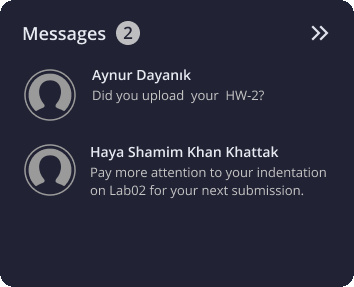
\includegraphics[width=0.46\textwidth]{messages_panel}
        \caption{Messages mini-panel}
        \label{fig:messages_panel}
    \end{wrapfigure}
    
    The messages panel (Figure \ref{fig:messages_panel}) serves the purpose of showing the user a brief outline of their unread messages
    without having to visit the full messages page. The user can click on any of the messages shown, or the right-pointing arrows on the top right,
    in order to visit their full messages page, where they can read and respond to messages.
    The calendar panel (located under the messages panel, see Figure \ref{fig:dashboard_full}) was not added in detailed manner
    to the design prototypes for the sake of simplicity.
    However, very plainly, its purpose is to show the user their assignment due dates visually by marking the days with due dates. 
    It does not have any advanced capabilities at all, and is not exactly intended to be interacted with.
    
    \pagebreak
    % After this point, you don't need to be worried about breaking the "Dashboard" section.
    
    \subsubsection{Messages}
    
    \begin{figure}[H]
        \centering
        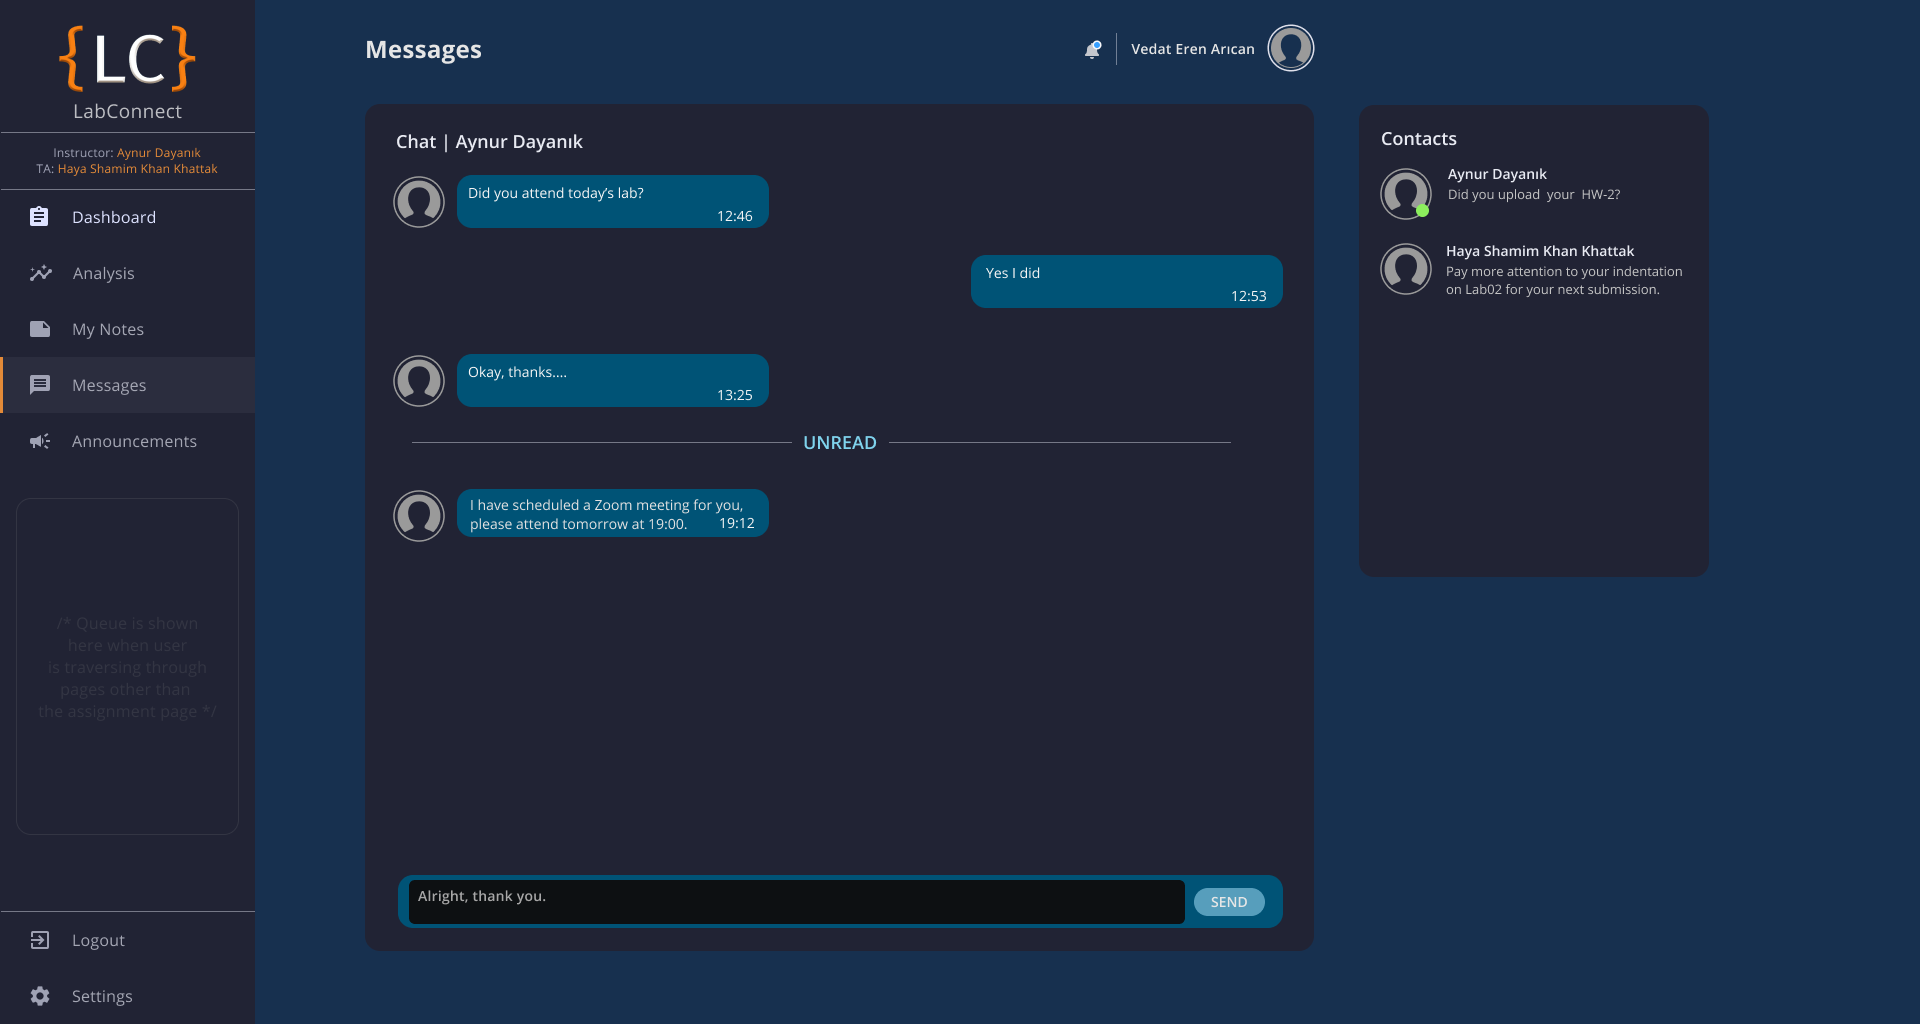
\includegraphics[width=\textwidth]{messages}
        \caption{Complete view of the messages UI}
        \label{fig:messages_full}
    \end{figure}
    
    Students, instructors and teacher assistants can send each other messages from the messages tab (Figure \ref{fig:messages_full}). By the overall design messages tab is fairly easy to use and
    self-explanatory. On the right hand side there is a contacts view which the registered contacts, contacts's online status and a small poriton of the last message is displayed.
    The conversation screen is displayed in the center item. Moreover, messages are displayed with the timestamp of the sending time and respondent's profile picture. 
    
    
    \pagebreak
    
    
    \subsection{Student-specific Views}
    
    This subsection illustrates the pages involved in the user experience of a student account.
    
    \subsubsection{Assignment Details}
    
    \begin{figure}[H]
        \centering
        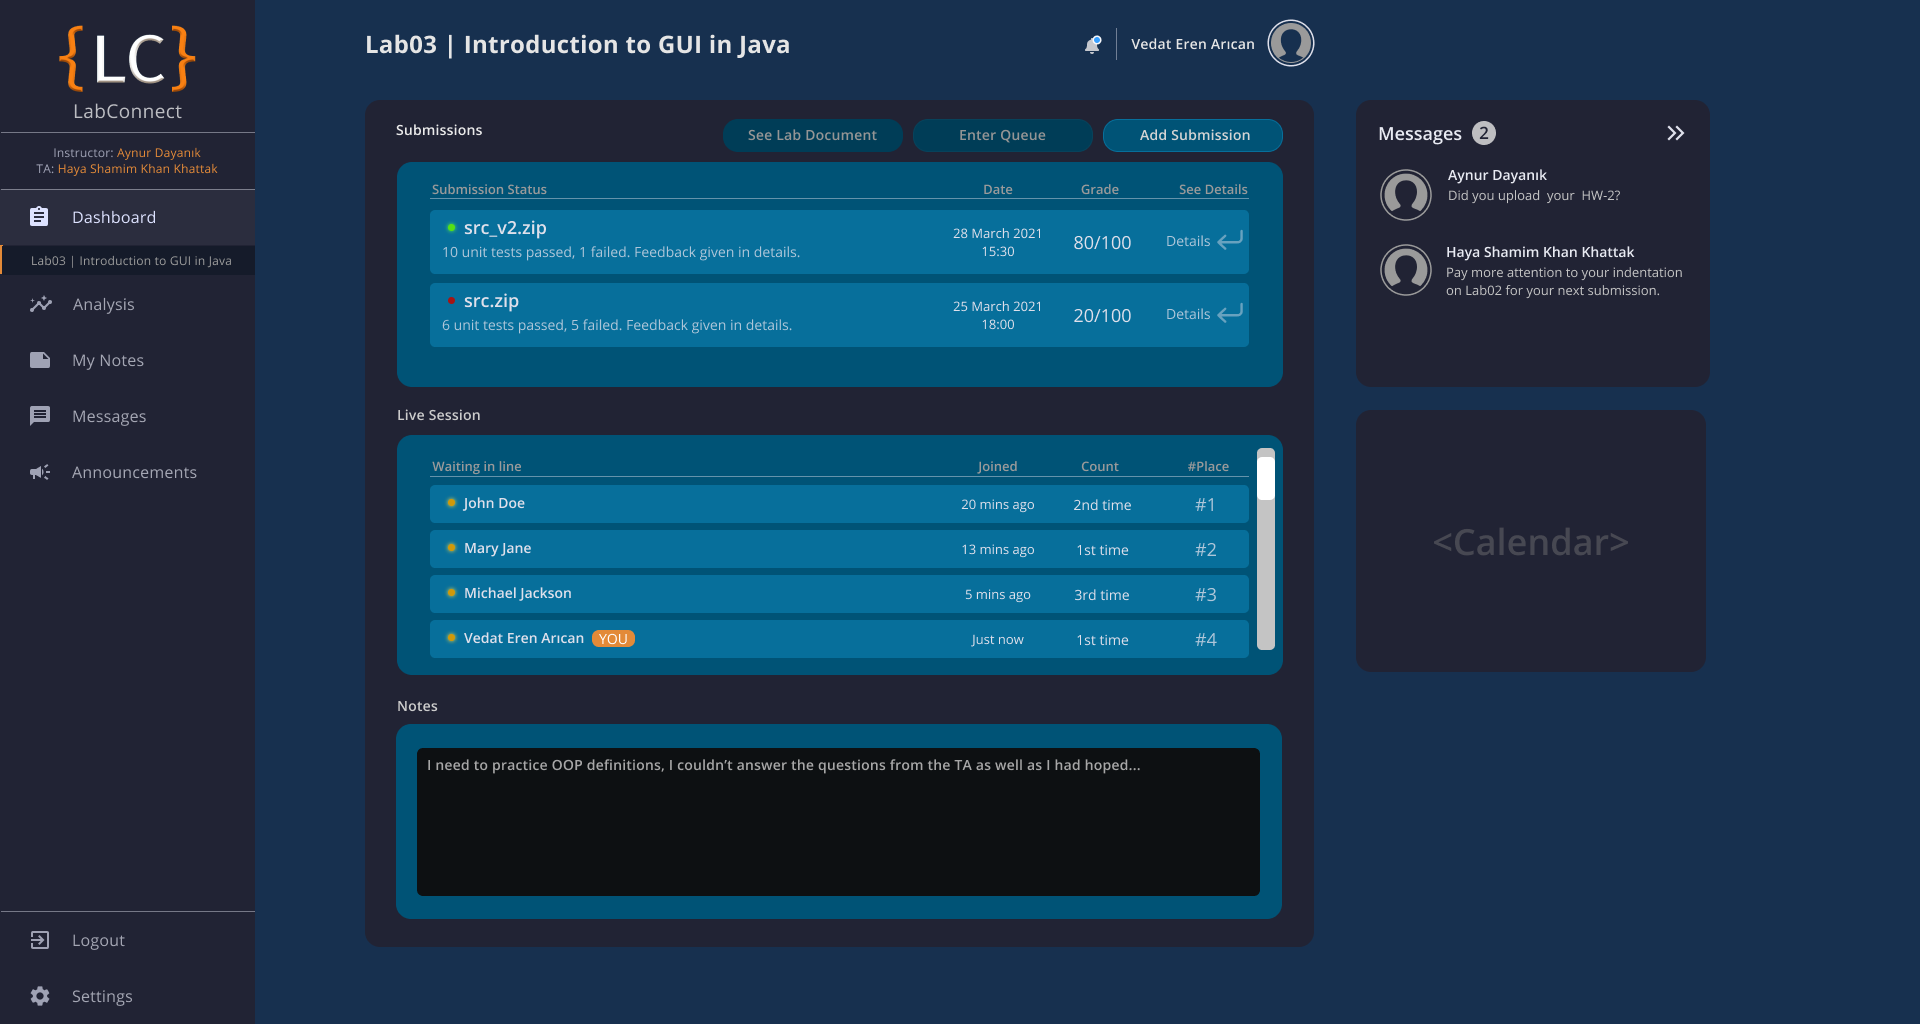
\includegraphics[width=\textwidth]{student_assignment_details}
        \caption{Complete view of the assignment details UI from a student's perspective}
        \label{fig:student_assignment_details_full}
    \end{figure}

    Once a student clicks on an assignment on the dashboard, the assignment details UI (Figure \ref{fig:student_assignment_details_full})
    is loaded. This interface contains three main sections, which are (from top to bottom):

    \begin{itemize}
      \item The ``Submissions'' section, where a student can check the status of their previous submissions and add new ones if necessary.
            The submissions are sorted based on the upload date. The student can view the upload date and grade for each submission,
            along with the submission's filename and a summary of the unit test results below that. Students can access detailed
            information about a submission by clicking the details button for that submission, which directs them to the
            assignment submission UI (see section \ref{student_submission}). To the left of the submission name is a circle colored either red or
            green, indicating the eligibility of the given submission for TA review. Buttons for adding a new submission, entering the
            review queue and viewing the assignment instructions are placed above this list.
      \item The ``Queue'' section, where the student can view the queue for their assigned TA if a live session is taking place. This section
            contains a scrollable list of students in the queue. The student can view the names of the people waiting in line, along with their
            place in the queue, their previous review count for this lab session and time elapsed since the given person joined the queue to get an idea
            of the waiting times.
      \item The ``Notes'' section, where the student can take personal notes about the given assignment. These notes can be accessed
            after the labs by clicking ``My Notes'' in the side bar. This functionality can be used as a journal of sorts, which can
            help the student keep track of subjects that they need to practice more.
    \end{itemize}
    
    \pagebreak
    
    \subsubsection{Assignment Submission} \label{student_submission}
    
    \begin{figure}[H]
        \centering
        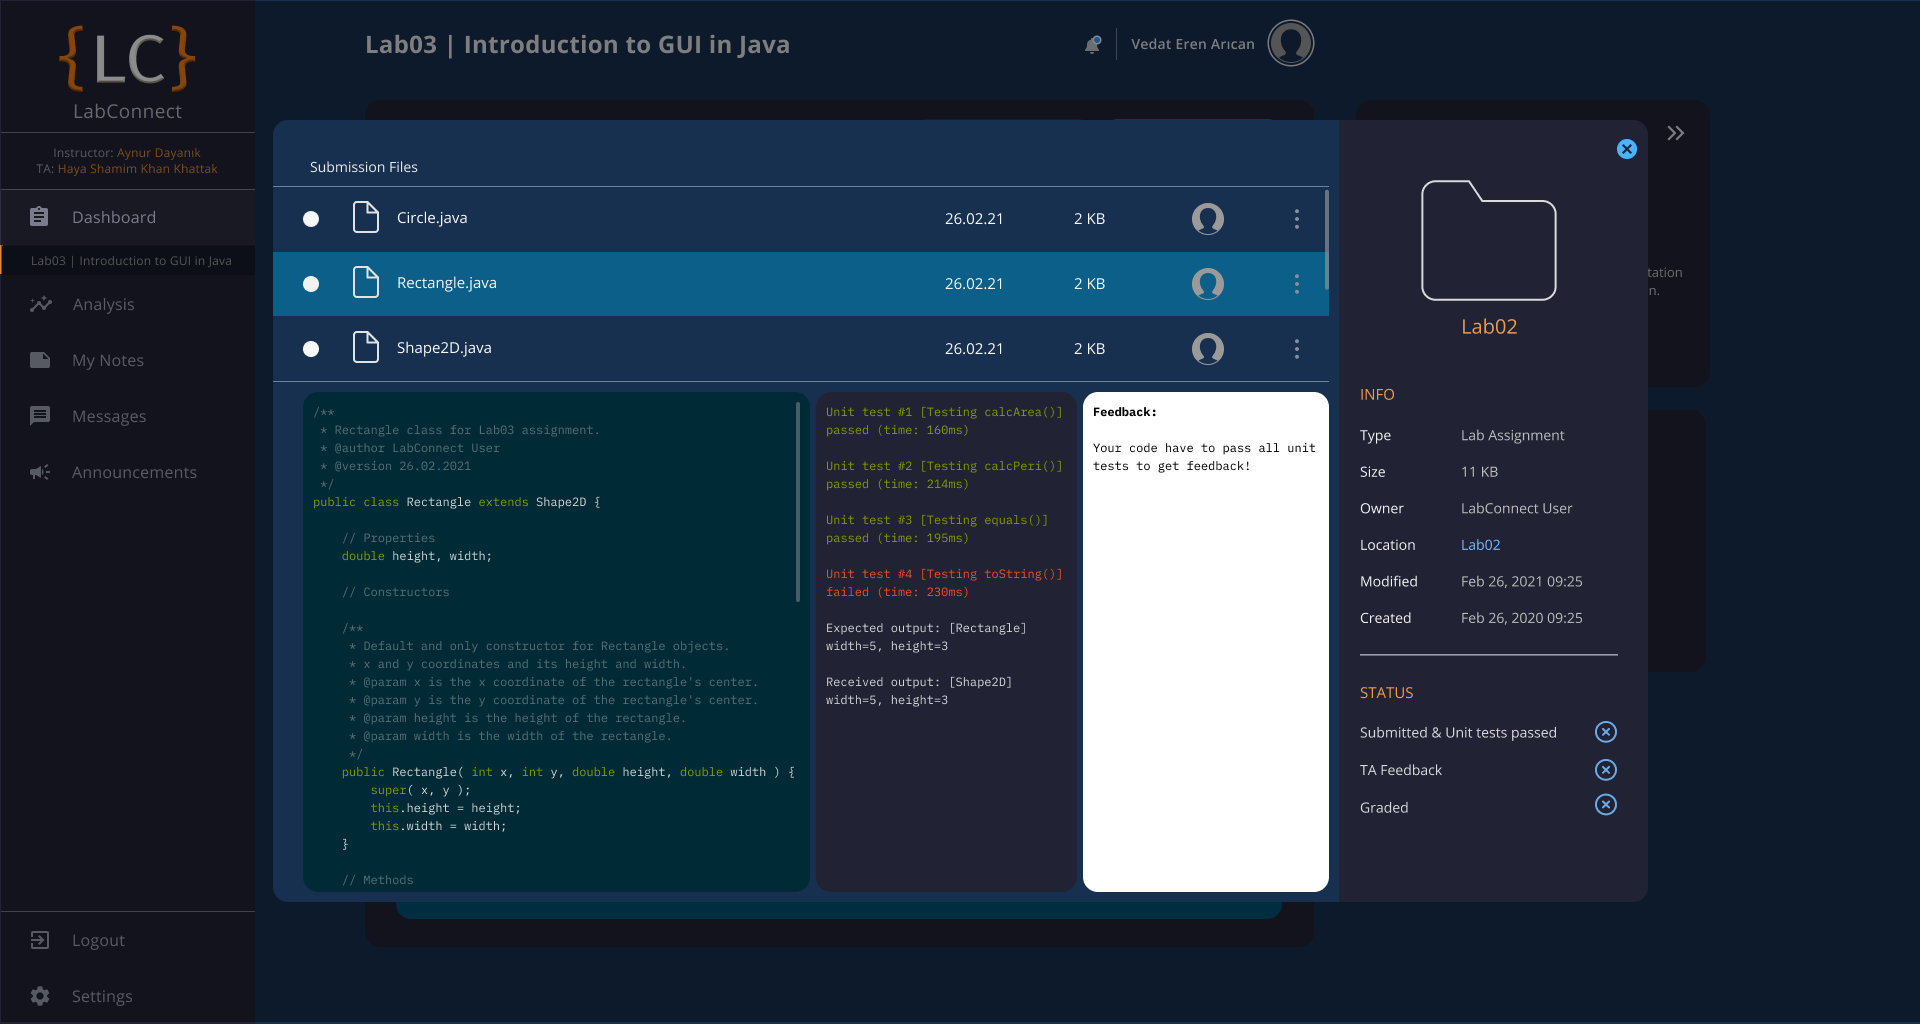
\includegraphics[width=\textwidth]{student_assignment_submission}
        \caption{Complete view of the assignment submission UI from a student's perspective}
        \label{fig:student_assignment_submission_full}
    \end{figure}

    On this screen (Figure \ref{fig:student_assignment_submission_full}), students can browse the files they have uploaded to the system as in a file explorer. 
    After selecting the reladted file at the top of the window, three different sections parts will appear below: the preview of the code contained in the file itself, 
    the outputs of the unit tests, and the TA's feedback to the file. Thanks to the code preview, students will be able to jump directly from the feedback 
    to the part or line the TA refers to. In the area where the output of the unit tests is available, students will be able to see which part of the code does not 
    work as desired and start to work on it immediately. Since TA feedback is clearly indicated on the same screen, students will be able to access the feedback they 
    receive for each file in a systematic and organized way.

    \pagebreak
    
    \subsubsection{Analysis}
    
    \begin{figure}[H]
        \centering
        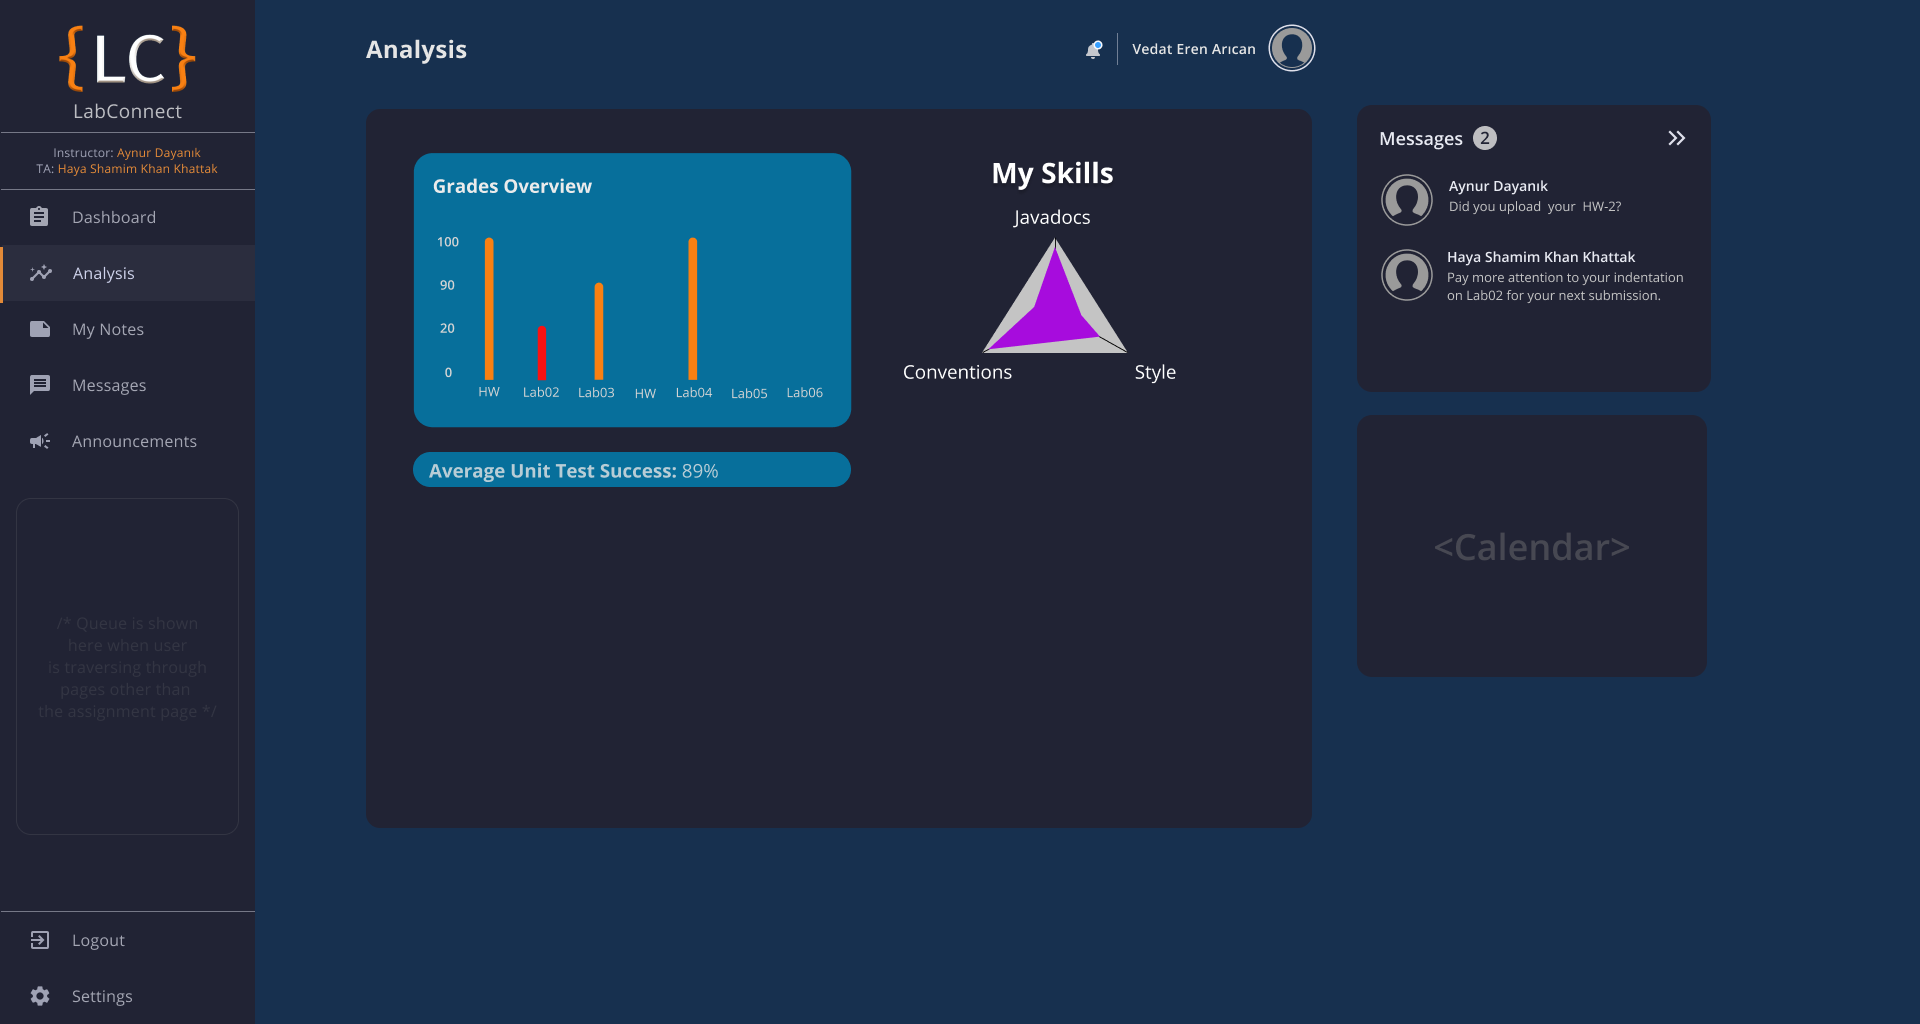
\includegraphics[width=\textwidth]{student_analysis}
        \caption{Complete view of the analysis UI from a student's perspective}
        \label{fig:student_analysis_full}
    \end{figure}
    
    In the analysis tab (Figure \ref{fig:student_analysis_full}). Students can see their individual performance mainly about the lab. assignments and homework.
    The performance criteria that is displayed is overview of last assignments as graph (in the graph the averages that are lower than the 
    pre-determined target will be indicated by another color), their documentation (Javadocs), compatibility with conventions and the style 
    (compatibility with course or other specific guidelines) as triangle chart and finally average success at unit testing (how often they 
    get stuck with standart and edge case testing [by percantage]).

    
    \pagebreak
    
    \subsubsection{Announcements}
    
    \begin{figure}[H]
        \centering
        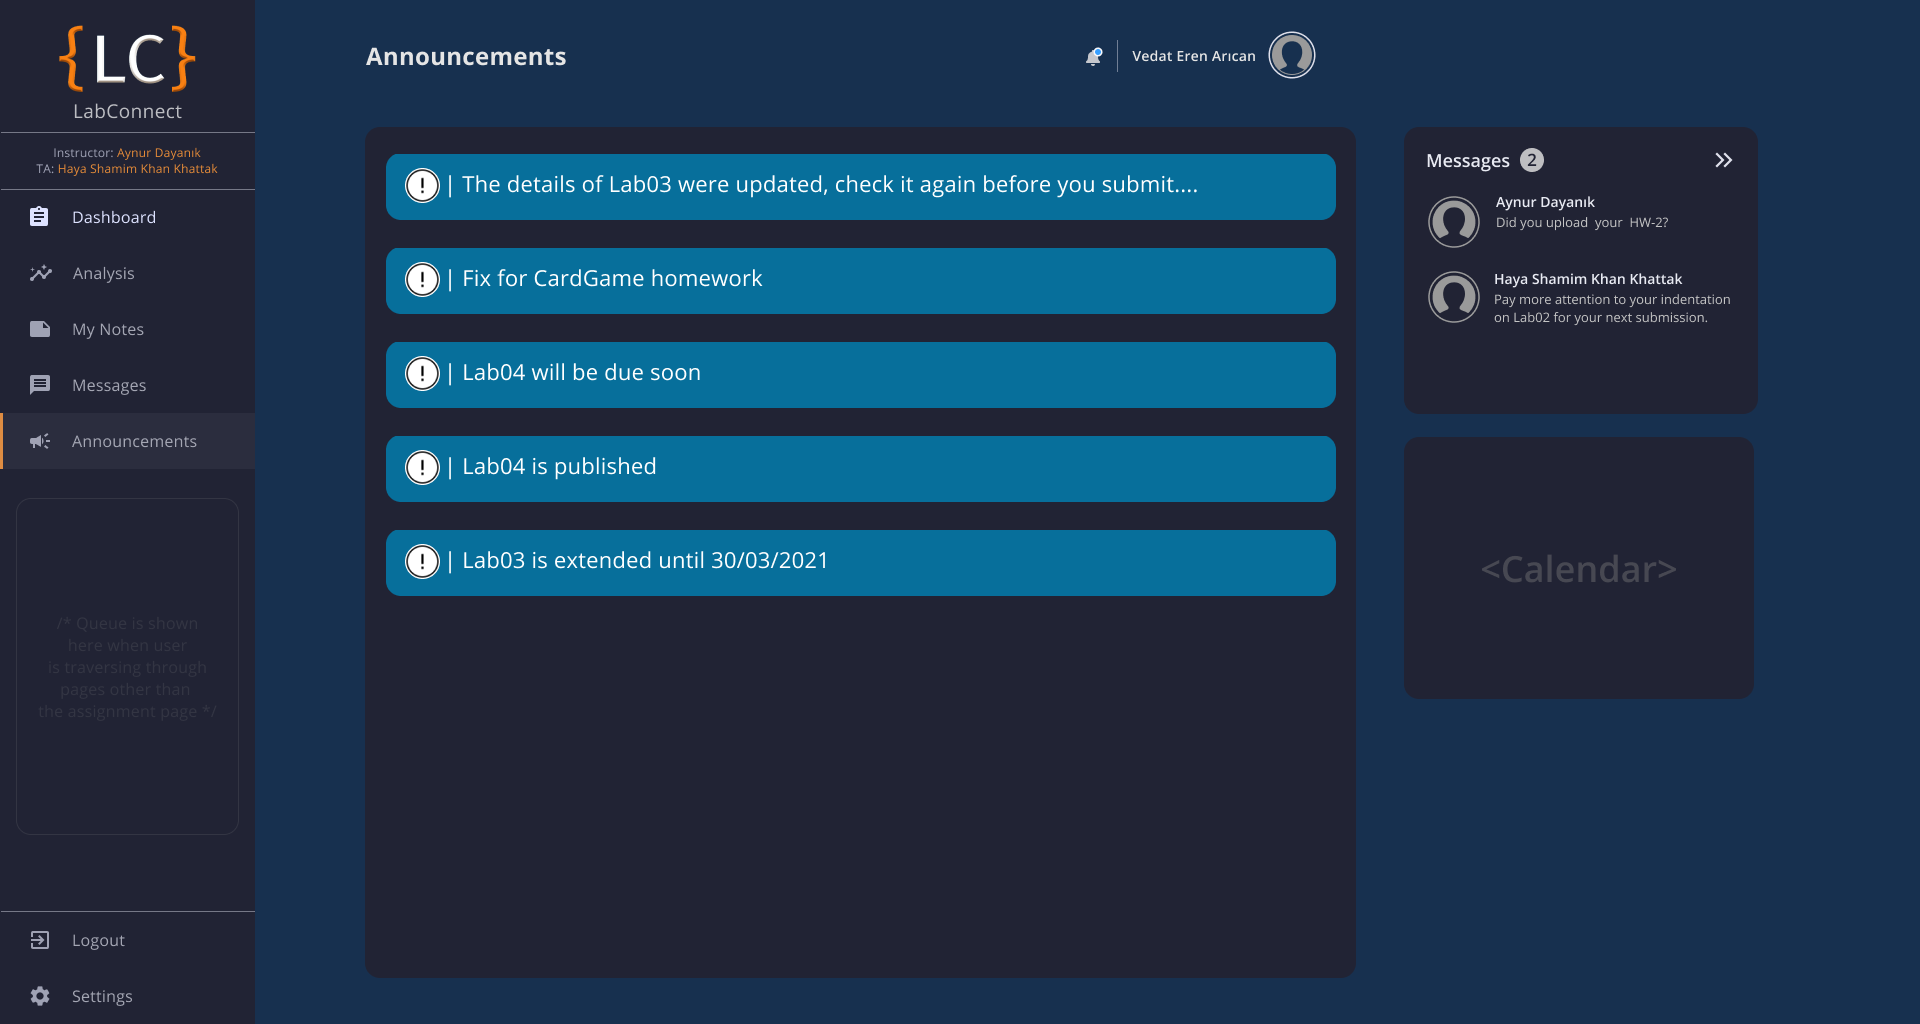
\includegraphics[width=\textwidth]{student_announcements}
        \caption{Complete view of the announcements UI from a student's perspective}
        \label{fig:student_announcements_full}
    \end{figure}
    
    In the announcements tab (Figure \ref{fig:student_announcements_full}) students can see the course related announcements which is posted by instructor. This tab is working simultanously
    with the bell icon at the top of the screen. Whenever a new announcement is made the bell icon will change in order to indicate the arrival of the 
    new announcement. When students click on the individual announcement the details of the announcement will be displayed as plain text.
    
    
    \pagebreak
    
    \subsubsection{Notes}
    
    \begin{figure}[H]
        \centering
        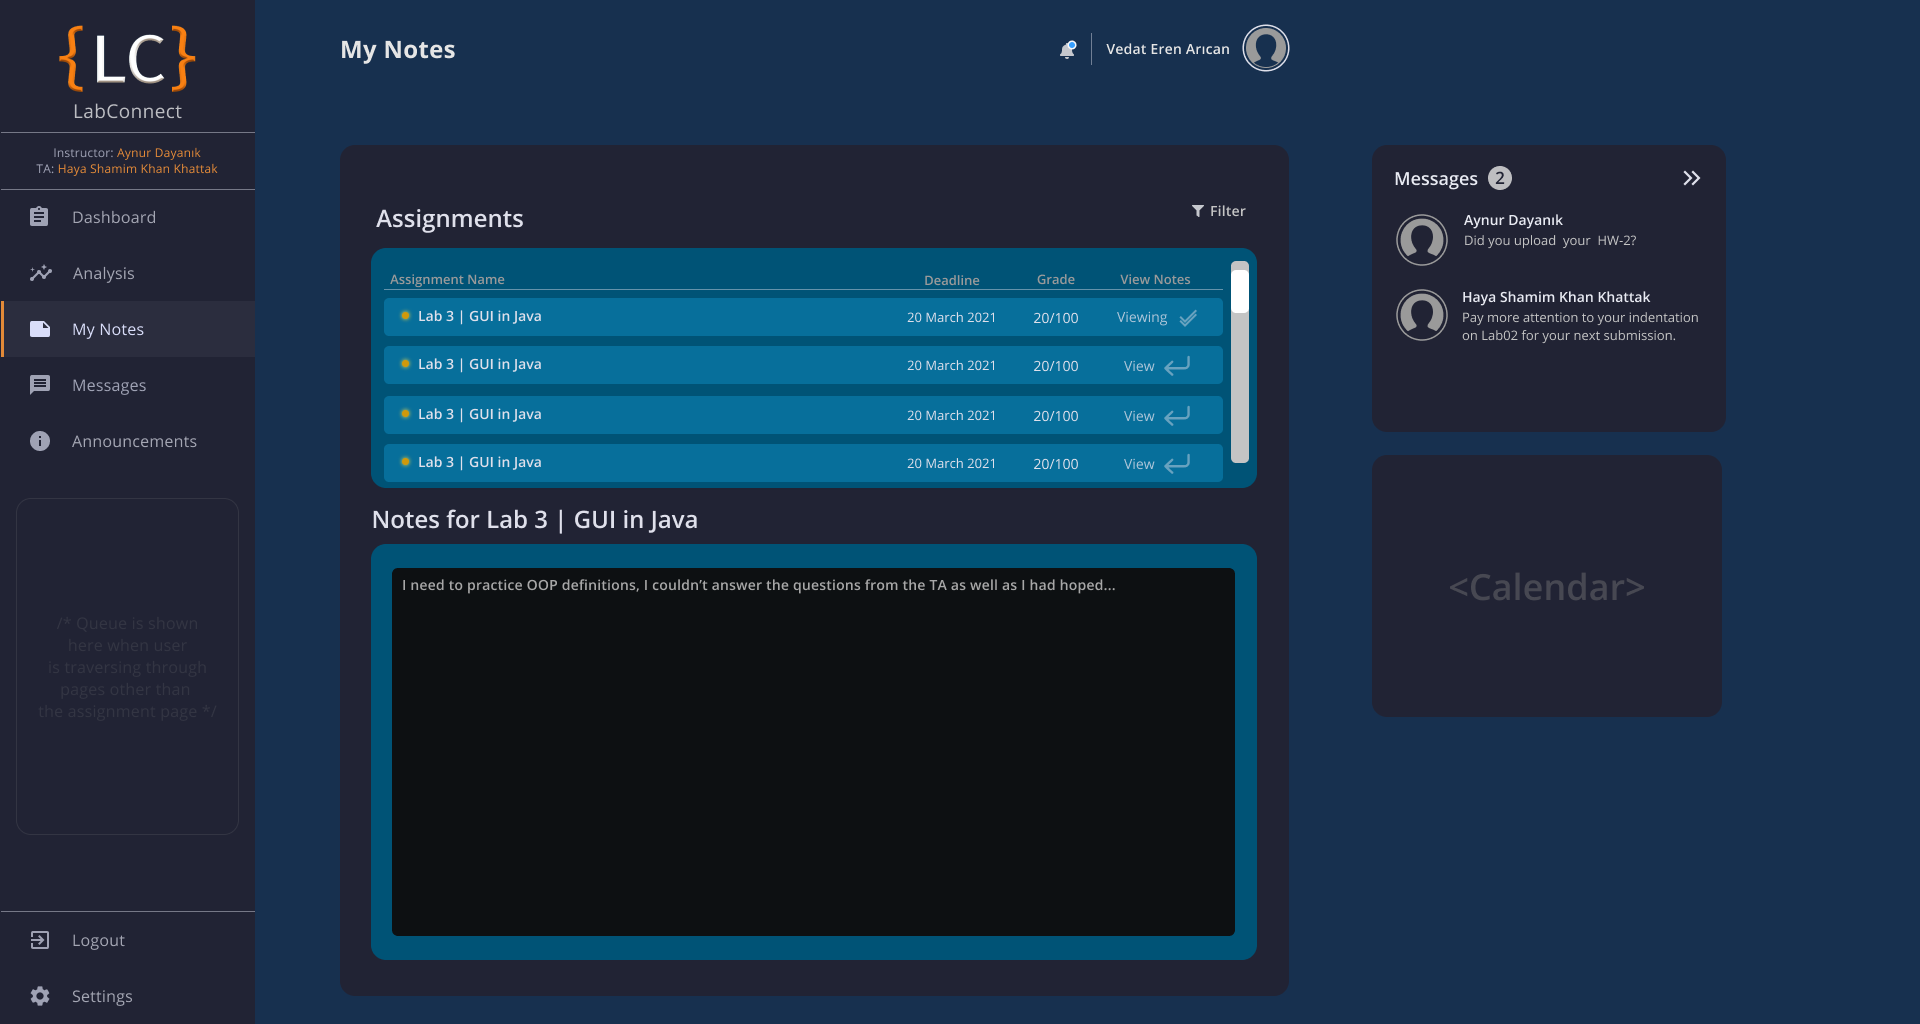
\includegraphics[width=\textwidth]{student_notes}
        \caption{Complete view of the notes UI from a student's perspective}
        \label{fig:student_notes_full}
    \end{figure}
    
    
    
    
    
    
    During code review taken by the TA, or a group work that is being held in the lab itself,
    the student would like a place for taking individual notes. These notes can be about their
    mistakes on the lab that is pointed out by the TA, or it can be about the project that the 
    students are doing in groups. LabConnect supplies students with a proper place where students
    can take notes in an organised manner and they have the chance to save them and take a look
    at them afterwards if needed. This enables them to have a proper way of organising their ideas
    and they prevent them from missing out the things the Ta mentioned or suggested about. In the
    program, the notes are organised in a way that they are distributed and saved based on the 
    assignment or the project itself. This way, their notes are well organised into subcategories
    based on the subject.
    
    
    
    
    
    \pagebreak
    
    
    \subsection{TA-specific Views}
    
    This subsection illustrates the pages involved in the user experience of a TA account.
    
    \subsubsection{Assignment Submission}
    
    \begin{figure}[H]
        \centering
        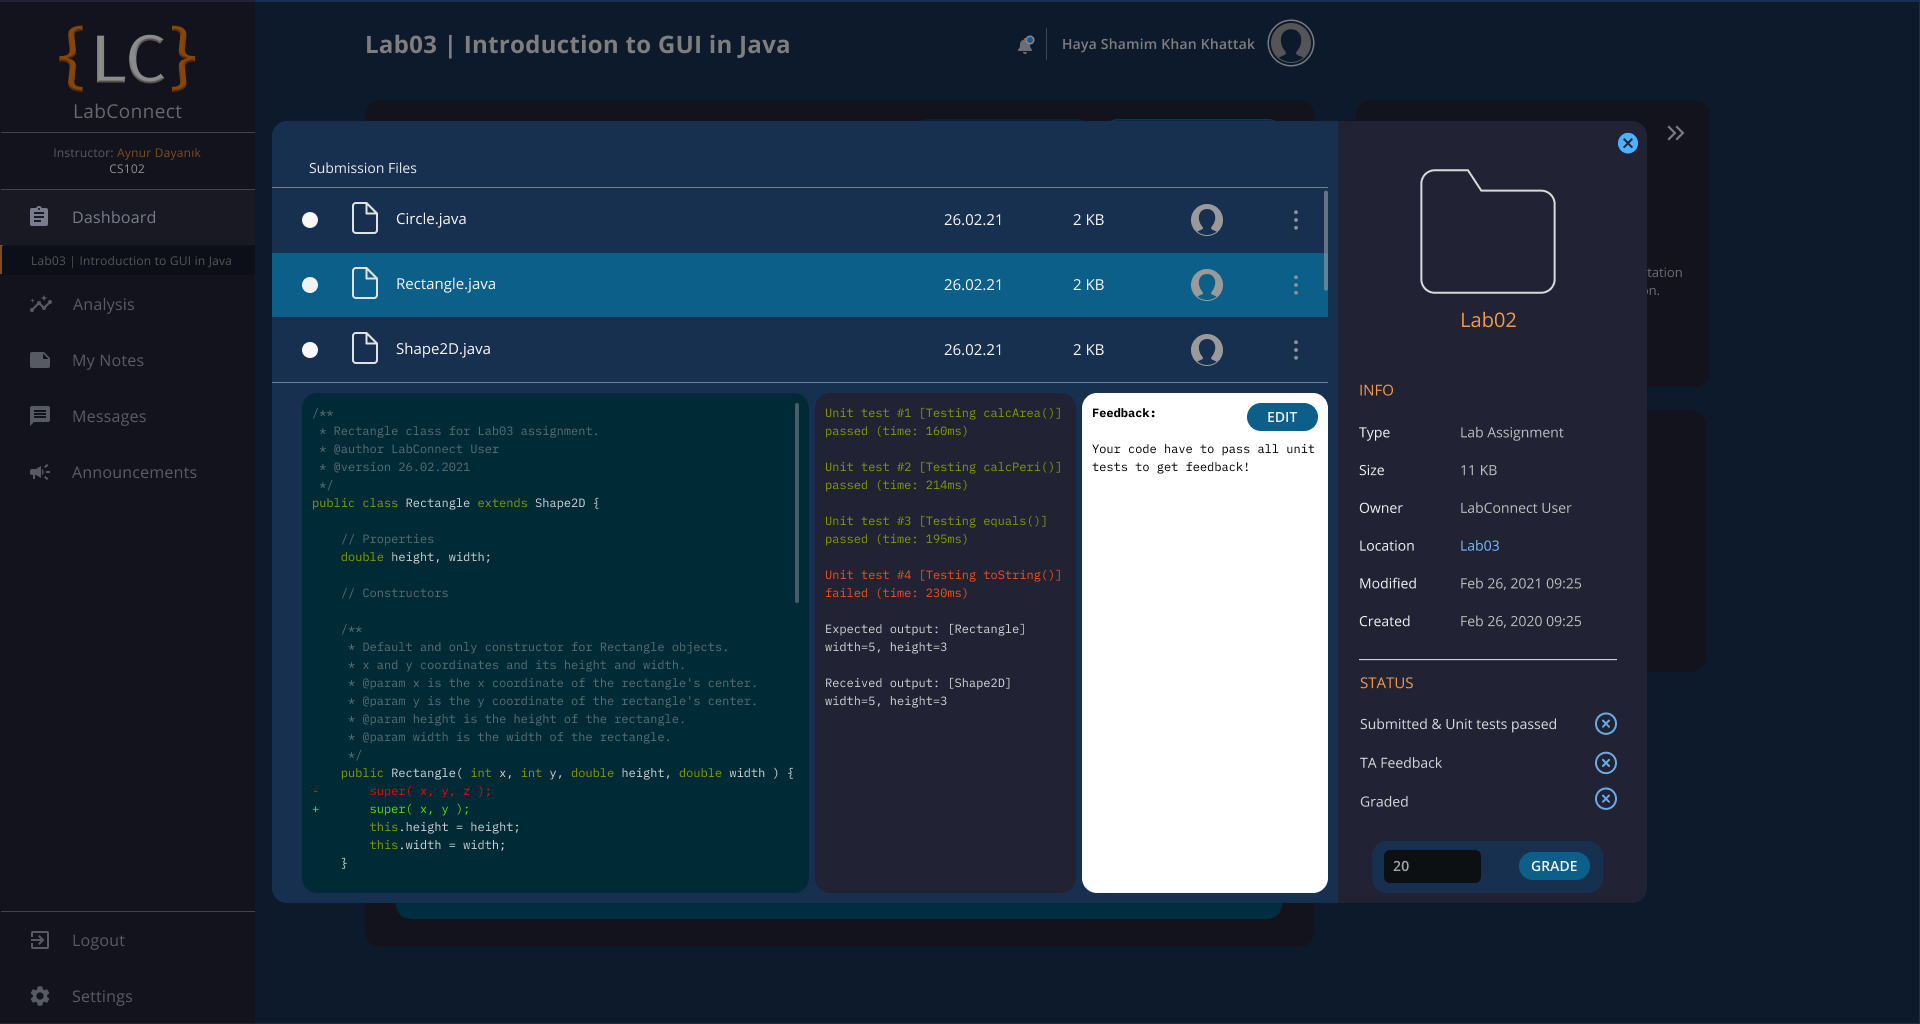
\includegraphics[width=\textwidth]{ta_assignment_submission}
        \caption{Complete view of the assignment submission UI from a TA's perspective}
        \label{fig:ta_assignment_submission_full}
    \end{figure}
    
    
    
    
    
    
    
    % TODO Write some details for the assignment submission "popup" (TA perspective)
    After the student has submitted their files to LabConnect. These files are available
    for the TAs by this tab. On top, the submitted files are seen and TA can choose between
    these files to browse through the source code itself on the left side of the panel, they
    can investigate on the results of the unit tests on the middle right of the screen, and
    they can comment on the individual works on the very right part of the page. This panel has
    everything the TA needs to look at and comment on the work done by the student. On the left,
    the TA is supplied with some information where they can do a quick check on the work. 
    For example, they can see the submission time of the file immidiately without leaving the
    scene, they can see whether all unit tests are passed for this work, or they can see whether
    this project is graded or not. If they haven't give any grades for the work (which is displayed
    on the right), they can immidately do this on the part bottom right. This interface saves 
    time for the TA since everything is integrated with each other so everything can be handled in
    the same page.
    
    
    
    
    
    \pagebreak
    
    \subsubsection{Ongoing Live Session}
     
    \begin{figure}[H]
        \centering
        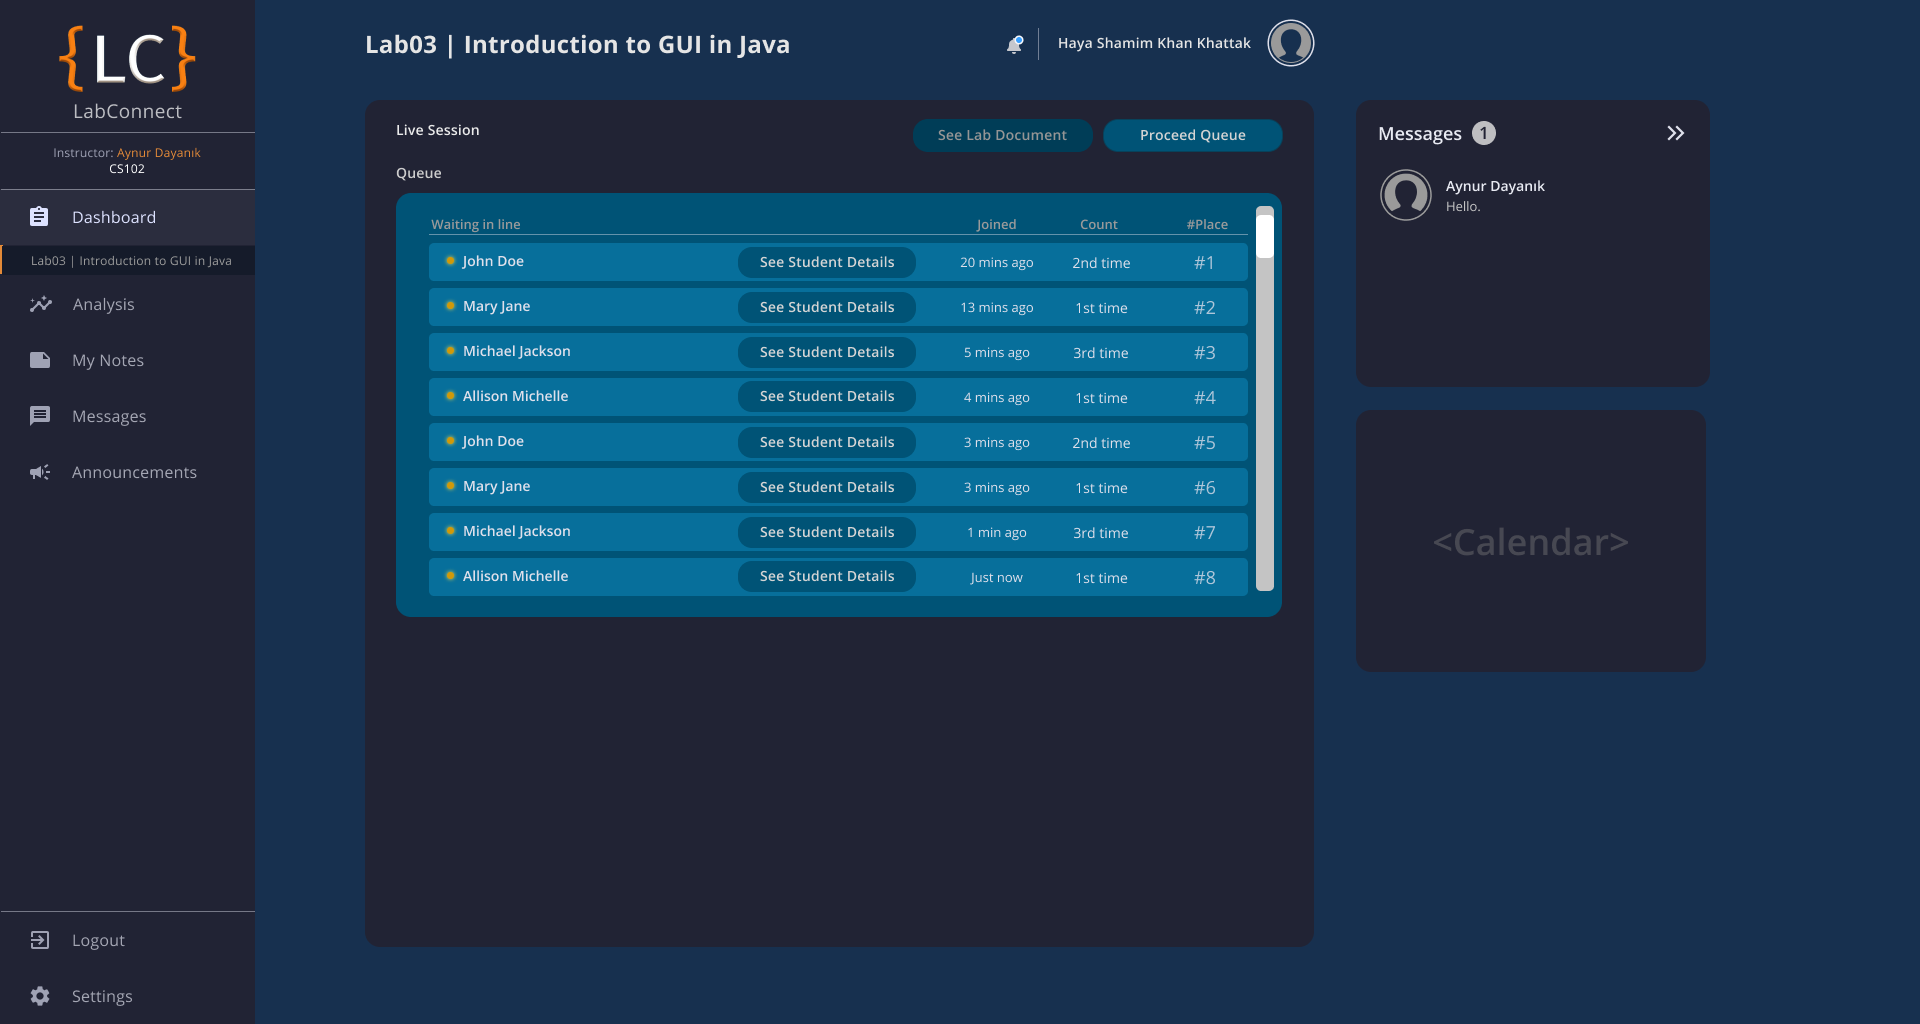
\includegraphics[width=\textwidth]{ta_live_session}
        \caption{Complete view of the live session UI from a TA's perspective}
        \label{fig:ta_live_session_full}
    \end{figure}
    

    
    
    
    % TODO Write some details for the live session page (TA perspective)
    
    
    
    
    
    
    \pagebreak
    
    
    \subsection{Instructor-specific Views}
    
    This subsection illustrates the pages involved in the user experience of an instructor account.
    
    \subsubsection{Announcements}
     
    \begin{figure}[H]
        \centering
        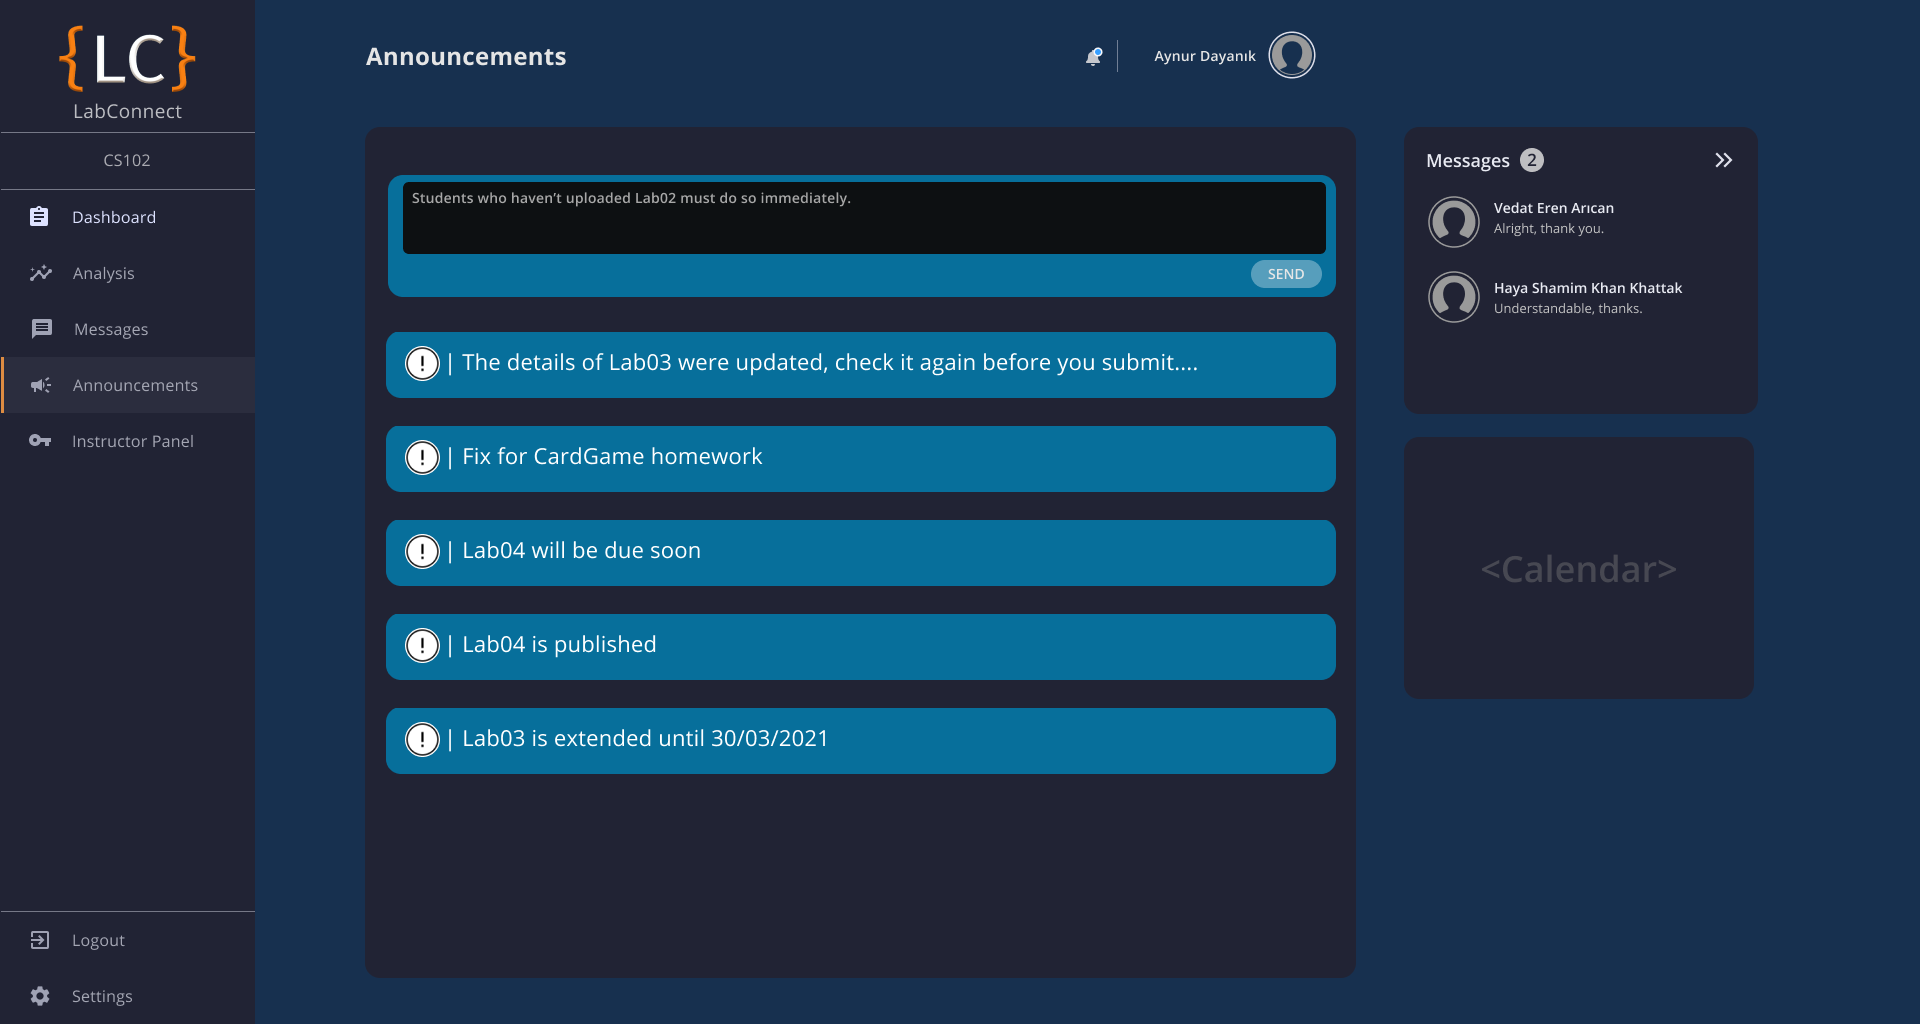
\includegraphics[width=\textwidth]{instructor_announcements}
        \caption{Complete view of the announcements UI from an instructor's perspective}
        \label{fig:instructor_announcements_full}
    \end{figure}
    

    
    
    
    
    
    % TODO Write some details for the announcements page (instructor perspective)
    
    
    
    
    
    \pagebreak
    
    \subsubsection{Instructor Panel}
    
    \begin{figure}[H]
        \centering
        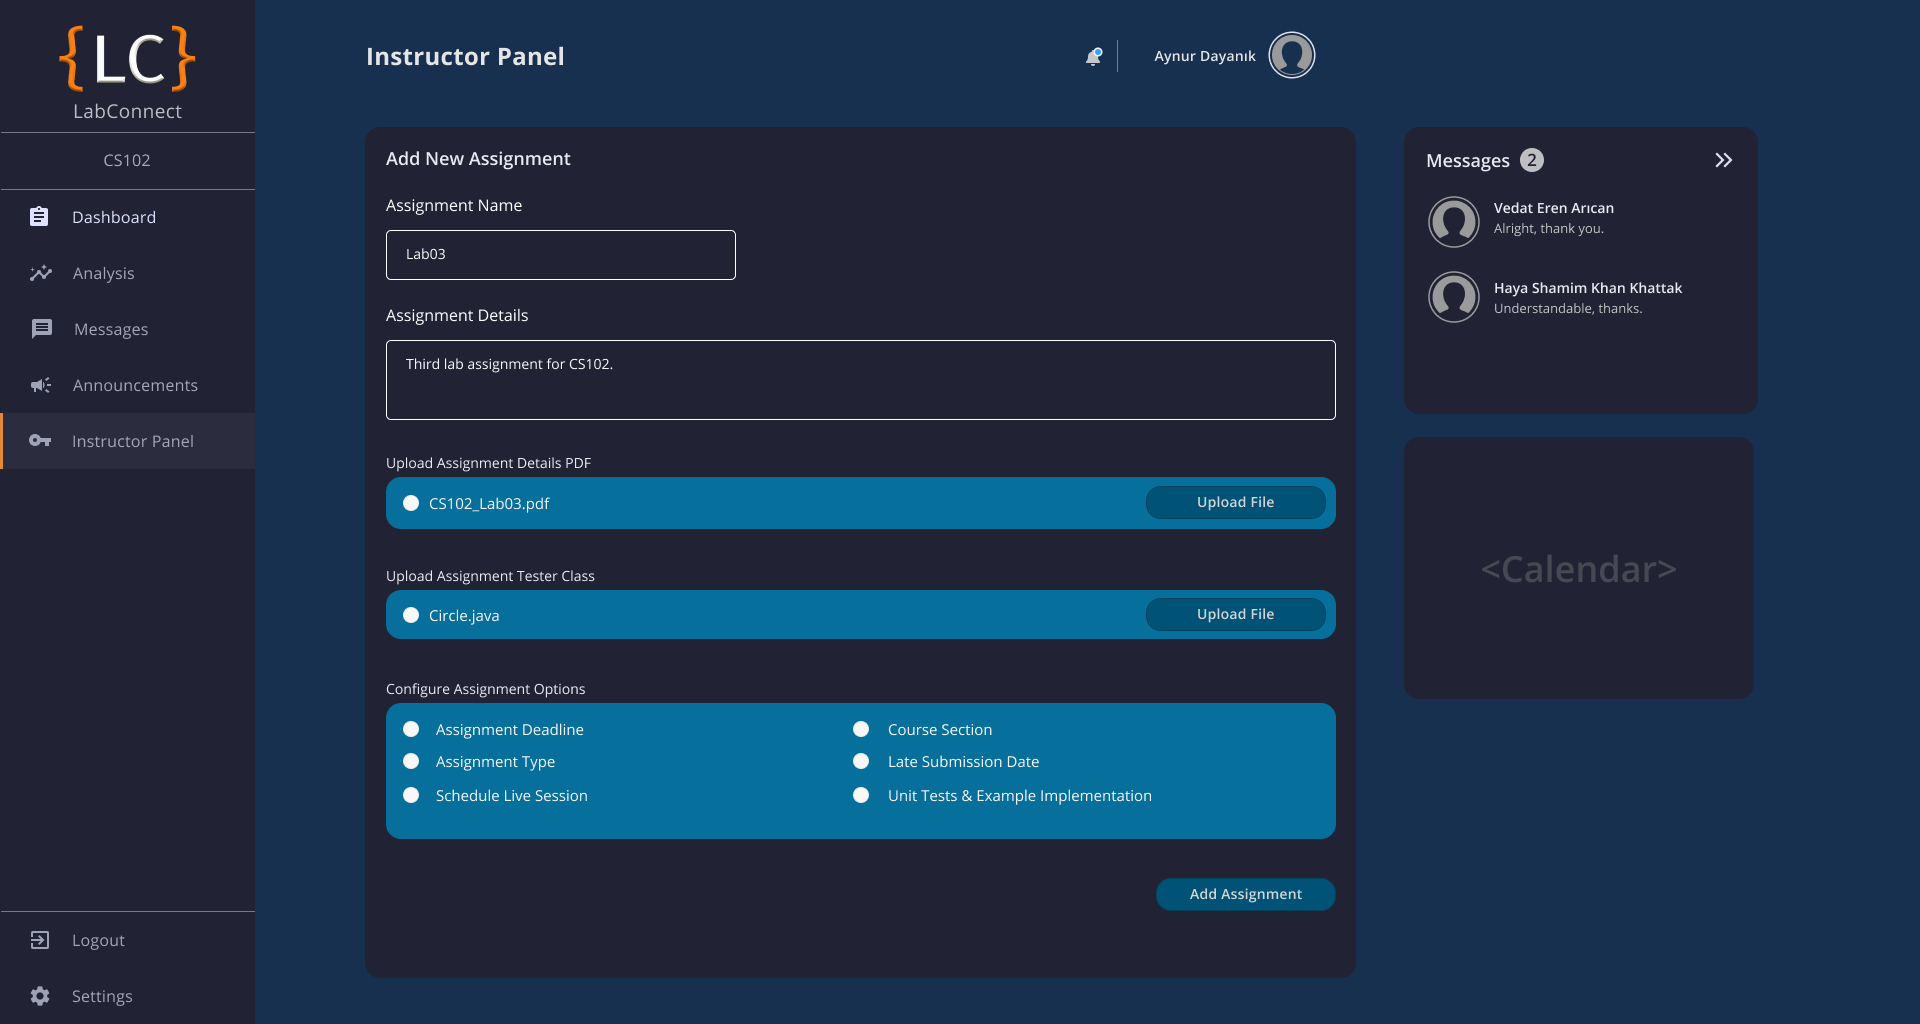
\includegraphics[width=\textwidth]{instructor_admin_panel}
        \caption{Complete view of the instructor panel UI from an instructor's perspective}
        \label{fig:instructor_admin_panel_full}
    \end{figure}
    
    
    
    
    
    
    % TODO Write some details for the instructor panel (instructor perspective)
    
    
    
    
    
    
    
    \pagebreak
    
    \subsubsection{Analysis}
    
    \begin{figure}[H]
        \centering
        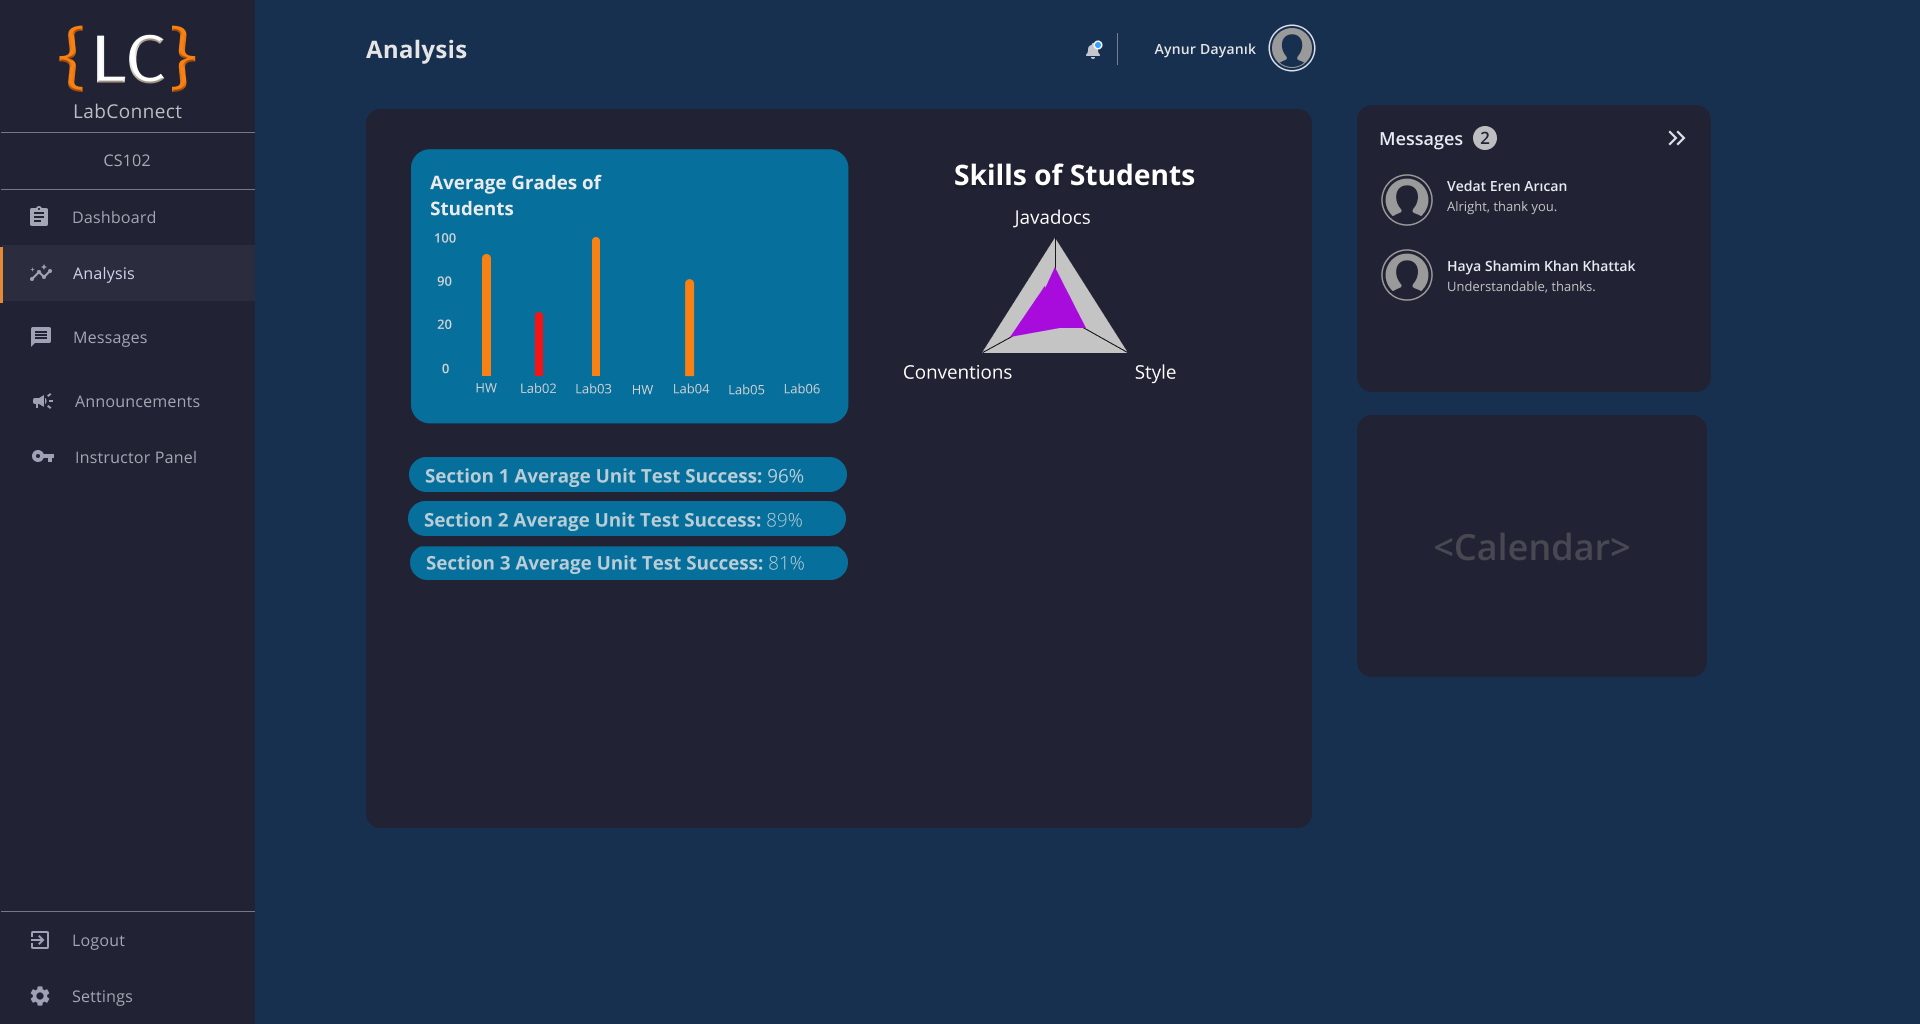
\includegraphics[width=\textwidth]{instructor_analysis}
        \caption{Complete view of the analysis UI from an instructor's perspective}
        \label{fig:instructor_analysis_full}
    \end{figure}

    In the analysis tab (Figure \ref{fig:instructor_analysis_full}) instructors can view the performance average of all sections. The performance criterias are similar with the ones that displayed in the student view.
    On the left corner of the center item, the average grades (average of all sections) of assignments are displayed as graph. In the graph the averages that are lower than the 
    pre-determined target will be indicated by another color. On the right corner the average skills of students which is based on documentation (Javadocs), compatibility with 
    conventions and the style (compatibility with course or other specific guidelines) as a triangle chart. Finally, on the left end corner of the center item, the average 
    success at unit tests of every section is displayed solely. 
    
    
    \pagebreak
    
    \section{Final Remarks}
    
    The user interface of LabConnect was designed while being conscious of the experiences we have been undergoing for the past two semesters of CS courses.
    The same care that we had put into compiling a list of features that we thought would alleviate many of the issues we had observed,
    was put into designing an interface such that users would not be facing the interface as an obstacle at any point during their usage.
    Striving to remain as simple and to-the-point as possible, as the UI design matures throughout the development timeline, the plan is
    to continue to have a focus on being UX-oriented. The design we have formulated is by no means unique, as countless web applications adopt 
    quite similar interfaces. However, rather than being seen as detrimental to the creativity of this design, we consider this wide usage 
    to be a testimony of the design being a viable option for user satisfaction. Additionally, many users may be content with the advantage of
    being familiar with the interface from the very start. 
    
    Also, for the sake of coverage, another point to address is our decision of basing our design on a dark color scheme. Though we are concerned that the psychological association of
    lighter colors with professional-looking reputable websites may surprise some users upon their initial visit, we also firmly recognize that the programmers
    of our day have a strong preference towards interfaces with colors that do not stress the eye. Considering the fact that our project caters quite specifically to
    a user base consisting of programmers, we think that picking a lighter color scheme would have been frustrating to the overwhelming proportion of users who will
    be 
    using this website among their otherwise dark-themed workspace. 
    Alas, we have determined it most sensible to put our efforts into developing a dark-mode interface, though we may choose to add the option of switching
    to a light-mode theme in the later stages of the project's development.

    % Not sure if a bibliography will be necessary for this report.
    % Remove later if there's no need.
    \pagebreak
    \printbibliography

\end{document}
